\newpage
\subsection{Content Server} \label{section:counter-replace-server}
This approach enforces users to log into a server and not relying on the verification response itself, but the returned content for the application, only accessible on successful verification.
This content cannot be guessed by \gls{luckypatcherg}.
A presentation of this approach is in figure~\ref{fig:contentServer}.
\newline
\begin{figure}[h]
    \centering
    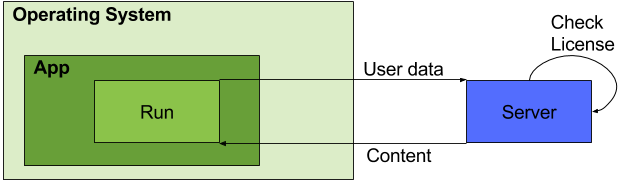
\includegraphics[width=1\textwidth]{data/contentServer.png}
    \caption{Abstraction of an application and a content server}
    \label{fig:contentServer}
\end{figure}
\newline
An implementation can be illustrated by looking at the application Spotify \cite{spotify} as an example.
Instead of verifying the license locally on the device, the user has to enter their credentials and send them to the server.
In case the credentials are valid, the user has the right to receive content.
The content, the music in this case, is no longer on the device itself, but streamed from the server.
The attacker still can circumvent the login process inside the application by manipulating the code.
Since the content is on the server, this content is not available inside the application until the user is authorized on the server.
Thus attacks on the application itself do not yield the desired result anymore.
\newline
\newline
In general, a content server is a solution against piracy, but it has downsides as well.
The first problem is that this architecture cannot be applied to all applications.
If there is no complex enough content that can be moved to the server, it doesn't work.
\newline
The second problem is the more complex overall architecture.
Instead of using Google's solution for handling the verification and only implementing the application logic on the device, a full size client server structure for the content has to be developed and implemented.
\newline
The third problem are the additional resources needed.
When outsourcing parts of the application on a server, money is needed for the server.
\newline
The fourth problem is the requirement for a permanent online connection.
It limits the freedom of users and creates additional internet traffic and costs.
This is not accepted by all users.
\newline
\newline
The content server mechanism protects the developers \gls{ip} when the core algorithm is moved to the server.
This prevents attackers not only from using the application for free, but also from reconstructing the core functionality and implementing it somewhere else.
